% Options for packages loaded elsewhere
\PassOptionsToPackage{unicode}{hyperref}
\PassOptionsToPackage{hyphens}{url}
\PassOptionsToPackage{dvipsnames,svgnames,x11names}{xcolor}
\documentclass[
  11pt,
]{article}
\usepackage{xcolor}
\usepackage[margin=25mm]{geometry}
\usepackage{amsmath,amssymb}
\setcounter{secnumdepth}{-\maxdimen} % remove section numbering
\usepackage{iftex}
\ifPDFTeX
  \usepackage[T1]{fontenc}
  \usepackage[utf8]{inputenc}
  \usepackage{textcomp} % provide euro and other symbols
\else % if luatex or xetex
  \usepackage{unicode-math} % this also loads fontspec
  \defaultfontfeatures{Scale=MatchLowercase}
  \defaultfontfeatures[\rmfamily]{Ligatures=TeX,Scale=1}
\fi
\usepackage{lmodern}
\ifPDFTeX\else
  % xetex/luatex font selection
\fi
% Use upquote if available, for straight quotes in verbatim environments
\IfFileExists{upquote.sty}{\usepackage{upquote}}{}
\IfFileExists{microtype.sty}{% use microtype if available
  \usepackage[]{microtype}
  \UseMicrotypeSet[protrusion]{basicmath} % disable protrusion for tt fonts
}{}
\makeatletter
\@ifundefined{KOMAClassName}{% if non-KOMA class
  \IfFileExists{parskip.sty}{%
    \usepackage{parskip}
  }{% else
    \setlength{\parindent}{0pt}
    \setlength{\parskip}{6pt plus 2pt minus 1pt}}
}{% if KOMA class
  \KOMAoptions{parskip=half}}
\makeatother
\usepackage{longtable,booktabs,array}
\usepackage{calc} % for calculating minipage widths
% Correct order of tables after \paragraph or \subparagraph
\usepackage{etoolbox}
\makeatletter
\patchcmd\longtable{\par}{\if@noskipsec\mbox{}\fi\par}{}{}
\makeatother
% Allow footnotes in longtable head/foot
\IfFileExists{footnotehyper.sty}{\usepackage{footnotehyper}}{\usepackage{footnote}}
\makesavenoteenv{longtable}
\usepackage{graphicx}
\makeatletter
\newsavebox\pandoc@box
\newcommand*\pandocbounded[1]{% scales image to fit in text height/width
  \sbox\pandoc@box{#1}%
  \Gscale@div\@tempa{\textheight}{\dimexpr\ht\pandoc@box+\dp\pandoc@box\relax}%
  \Gscale@div\@tempb{\linewidth}{\wd\pandoc@box}%
  \ifdim\@tempb\p@<\@tempa\p@\let\@tempa\@tempb\fi% select the smaller of both
  \ifdim\@tempa\p@<\p@\scalebox{\@tempa}{\usebox\pandoc@box}%
  \else\usebox{\pandoc@box}%
  \fi%
}
% Set default figure placement to htbp
\def\fps@figure{htbp}
\makeatother
\setlength{\emergencystretch}{3em} % prevent overfull lines
\providecommand{\tightlist}{%
  \setlength{\itemsep}{0pt}\setlength{\parskip}{0pt}}
\usepackage{bookmark}
\IfFileExists{xurl.sty}{\usepackage{xurl}}{} % add URL line breaks if available
\urlstyle{same}
\hypersetup{
  pdftitle={Constraint Torques at the Wrist: Grip Geometry, Energy Transfer and Face Control},
  pdfauthor={Dieter Butz},
  colorlinks=true,
  linkcolor={Maroon},
  filecolor={Maroon},
  citecolor={Blue},
  urlcolor={Blue},
  pdfcreator={LaTeX via pandoc}}

\title{Constraint Torques at the Wrist: Grip Geometry, Energy Transfer
and Face Control}
\author{Dieter Butz}
\date{Revised September 8, 2026}

\begin{document}
\maketitle

{
\hypersetup{linkcolor=}
\setcounter{tocdepth}{2}
\tableofcontents
}
This print companion preserves the original manuscript's author credit
and follows the corrected AffineDrift web article. Its idealized
derivations support a testable hypothesis; they do not establish a human
grip ranking.

\section{Abstract}\label{abstract}

Grip geometry can change how the golfer's motion and forces affect the
clubface. Understanding that effect requires more than resolving a
torque into two axes. The wrist's allowed motion determines its reaction
loads; the hand--club attachment transforms those loads; the club's
inertia and moving support determine its response; and the
face-orientation map determines which response matters at impact. Muscle
action, compliance and correlations between disturbances enter the same
chain. This article derives those connections using an ideal two-axis
wrist model, then identifies the measurements needed to qualify it. The
result is a testable grip-geometry hypothesis, not a demonstrated
ranking of finger and palm grips. Mechanical identities and illustrative
numerical examples are verified here; human performance and the author's
historical Simscape model are not validated by those checks.

\section{In Plain Language}\label{in-plain-language}

A joint can pass a load between body segments without behaving like an
extra motor. Changing how the club sits in the hand can change the
motion that this load produces. But a load that is less disruptive in
one configuration may become larger there, and the golfer may change
muscle action at the same time. The useful question is therefore:
\textbf{which measured grip geometry produces the desired club delivery,
with manageable effort and sensitivity, for this golfer?} The equations
below make each part of that question explicit.

\section{Introduction}\label{introduction}

The investigation began with a concrete simulation problem. A model was
driven with prescribed joint motion, and the joint reported forces and
torques. Could those recorded values be fed back as actuator inputs to
reproduce the motion in forward dynamics? The obstacle was that a
measured joint wrench and a set of actuator inputs are different
quantities. A joint can report three torque components while having only
two rotational coordinates. Some of its load enforces the joint geometry
rather than driving an independent rotation.

That observation motivates a broader golf question. Does the hand--club
attachment direct these loads into motion that develops useful clubhead
speed, or into motion that makes face control more sensitive? This is a
worthwhile mechanical hypothesis. Its answer depends jointly on
geometry, dynamics and the task. We will retain the question while
replacing claims of automatic transmission efficiency, inevitable
variability accumulation and universal grip superiority with quantities
that can actually be calculated and tested.

\subsection{The Wrist as a Universal
Joint}\label{the-wrist-as-a-universal-joint}

We distinguish the \textbf{wrist complex} from the \textbf{forearm's
radioulnar joints}. Flexion--extension and radial--ulnar deviation
describe two prominent directions of hand motion relative to the
forearm. Pronation--supination involves the radius and ulna and changes
the frame carried to the wrist. It should be modeled at the appropriate
forearm joints, not counted as an unactuated third wrist coordinate
after it has already been prohibited by a two-coordinate model.

The ideal wrist used here consists of two intersecting revolute axes.
Near a chosen neutral posture, associate flexion--extension with a
mediolateral axis and deviation with an approximately dorsopalmar axis.
Declare the anatomical calibration and signs for the particular limb.
These are modeling coordinates, not a claim that anatomical or
mechanical axes remain perfectly perpendicular and fixed throughout a
swing. Crisco and colleagues found oblique mechanical axes in a
six-cadaver-wrist study; their separate in-vivo study examined carpal
kinematics during dart-throwing motions. Neither study validates the
present golf model.
\href{https://pubmed.ncbi.nlm.nih.gov/21248214/}{Crisco et al., 2011},
\href{https://pubmed.ncbi.nlm.nih.gov/16322624/}{Crisco et al., 2005}.

\subsection{Limitations of the 2-DOF Wrist
Model}\label{limitations-of-the-2-dof-wrist-model}

A rigid joint is an approximation to motion under specified loads and
time scales. It can be useful when omitted relative motions have
negligible influence on the output being studied. That must be checked,
especially for tissue loads, contact transients and impact. A compliant
extension introduces extra states, constitutive parameters and possibly
activation-dependent stiffness. Calling an approximation ``rigid''
neither validates it nor makes it inherently invalid.

Two coordinates with two independent generalized torque inputs describe
a locally fully actuated wrist subsystem. Underactuation must instead be
assessed on the independent coordinates of the complete model, including
its floating base, contacts and actuator map. This is also a
\textbf{spatial} model: a two-axis joint is not a planar swing simply
because it has two rotational coordinates. Planar tests elsewhere in the
project cannot validate its out-of-plane face-orientation predictions.

\section{Universal Joints and Constraint
Torques}\label{universal-joints-and-constraint-torques}

\subsection{Mechanical Properties of Universal
Joints}\label{mechanical-properties-of-universal-joints}

The perpendicular axes in a universal joint belong to its cross pins.
The centerlines of the connected shafts can form a range of bend angles;
they are not required to be perpendicular. Furthermore, a freely moving
two-axis relative joint and a driveshaft held in two fixed bearings are
different mechanisms. The bearings impose additional constraints. The
familiar Cardan speed-ratio formula describes the latter assembly and is
derived separately below. It cannot be assigned directly to wrist
flexion and grip angle.

Let \(R={}^{F}R_H=R_x(\phi)R_y(\psi)\) map hand-frame vectors into the
forearm frame. At the joint's common point, the two allowed relative
angular velocity directions, expressed in the forearm frame, are

\[
\mathbf a=\mathbf e_x,\qquad
\mathbf b=R_x(\phi)\mathbf e_y,\qquad
\boldsymbol\omega_{H/F}=\mathbf a\dot\phi+\mathbf b\dot\psi.
\]

The ideal reaction couple must do zero power against every allowed
relative angular velocity. Thus it lies along the reciprocal direction

\[
\mathbf n_c=\mathbf a\times\mathbf b=R_x(\phi)\mathbf e_z,
\qquad \boldsymbol\tau_c=\lambda_r\mathbf n_c,
\qquad \mathbf n_c^T\boldsymbol\omega_{H/F}=0.
\]

For this convention a local holonomic orientation constraint is
\(\mathbf e_x^TR\mathbf e_y=0\). Its derivative gives the same
instantaneous restriction. The joint also imposes three translational
constraints at the common point, whose reactions are forces. If a wrench
is reported at a different point, those forces contribute an additional
moment.

\subsection{Derivation for the Wrist Universal
Joint}\label{derivation-for-the-wrist-universal-joint}

At \(\phi=30^\circ\), \(\psi=20^\circ\), the reciprocal unit direction
is

\[
{}^F\mathbf n_c=(0,-0.5,0.866025)^T,
\qquad
{}^H\mathbf n_c=R^T{}^F\mathbf n_c=(-0.342020,0,0.939693)^T.
\]

It is generally neither a fixed forearm \(z\)-axis nor a fixed hand
\(z\)-axis. The constraint does not say that a chosen Euler angle rate
or the forearm-frame component \(\omega_z\) vanishes. For example, the
allowed deviation direction \(\mathbf b=(0,\cos\phi,\sin\phi)^T\) has a
nonzero \(z\) component when the wrist is flexed. Confusing coordinate
rates with angular-velocity components would therefore label permitted
motion ``constrained.''

Because \(\mathbf a\) and \(\mathbf b\) are orthogonal unit vectors,
this joint's \(3\times2\) angular-velocity Jacobian has rank two.
Straight shaft alignment does not cause gimbal lock in this model.
Singularities of a supported driveshaft assembly, an Euler chart, and a
chosen golf task require their own analyses. They are not
interchangeable.

\begin{figure}
\centering
\pandocbounded{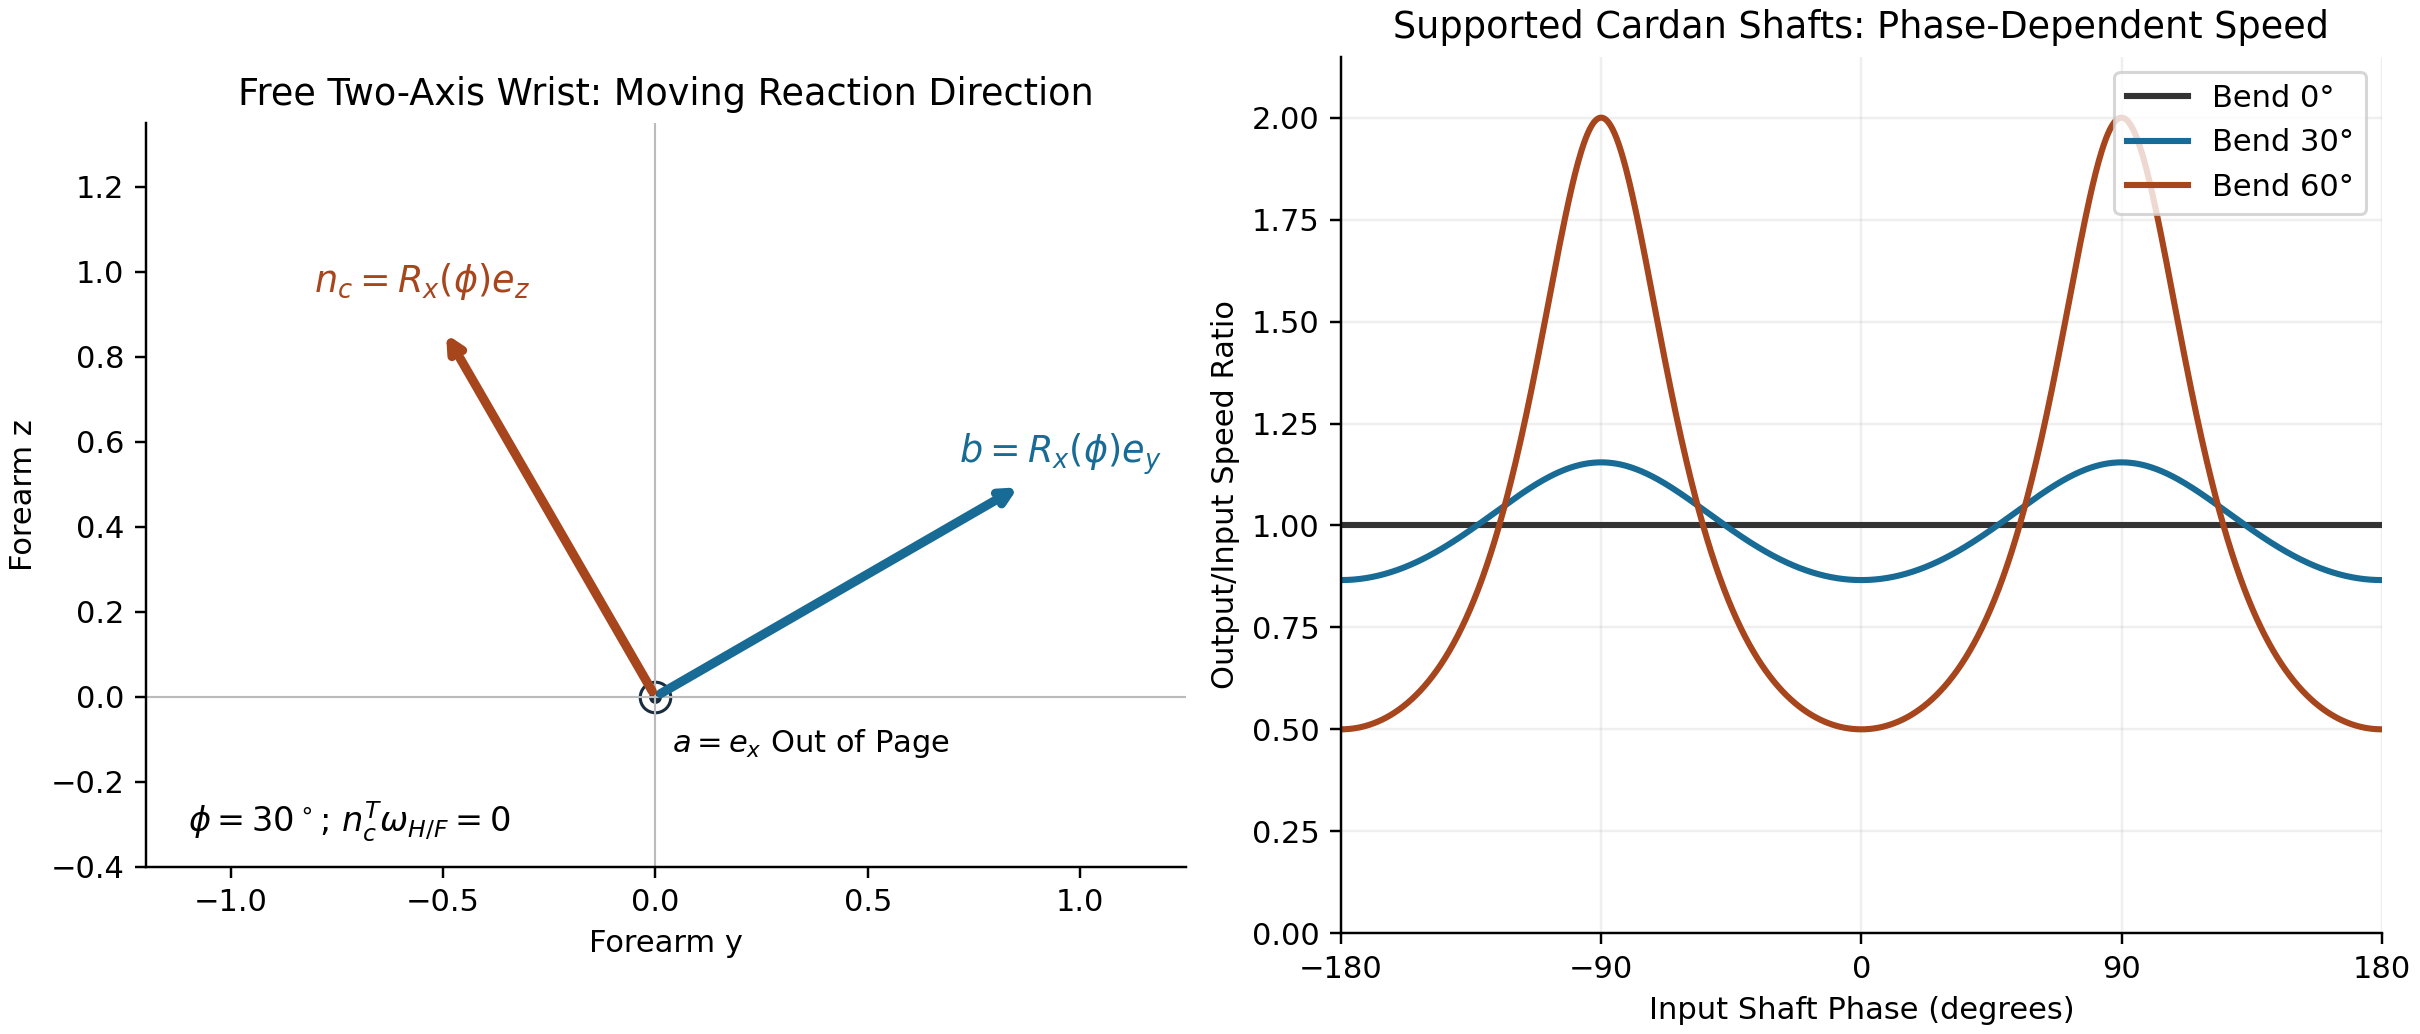
\includegraphics[keepaspectratio]{wrist-mechanisms.png}}
\caption{Two Different Mechanisms}
\end{figure}

The left panel shows the freely moving ideal wrist. The right panel
includes fixed shaft supports and therefore describes a different
mechanism. Its phase is not an anatomical wrist angle; the two panels
must not be identified by matching their angle symbols.

\subsection{Theoretical Formulation of Constraint
Torques}\label{theoretical-formulation-of-constraint-torques}

Use redundant local generalized coordinates \(\mathbf q\in\mathbb R^n\),
an independent constraint Jacobian \(A\in\mathbb R^{k\times n}\), and an
actuator map \(B\in\mathbb R^{n\times m}\). For stationary ideal
constraints,

\[
M\ddot{\mathbf q}+\mathbf h
=B\mathbf u+\mathbf f+A^T\boldsymbol\lambda,
\qquad A\dot{\mathbf q}=0.
\]

\(M\) is positive definite in this coordinate chart. The bias
\(\mathbf h\) includes gravity and velocity-dependent inertial terms;
\(\mathbf f\) contains other declared generalized forces, including
modeled passive forces if they are not placed in \(\mathbf h\). Use one
convention consistently. The components of \(\boldsymbol\lambda\) are
multipliers, not automatically anatomical torque components: their units
and meaning depend on how the constraint equations are scaled. The
physical generalized reaction is \(A^T\boldsymbol\lambda\).

Differentiate the velocity constraint and substitute the dynamics:

\[
AM^{-1}A^T\boldsymbol\lambda
=-\dot A\dot{\mathbf q}-AM^{-1}(B\mathbf u+\mathbf f-\mathbf h).
\]

With independent rows of \(A\), the left matrix is positive definite.
Solve this system rather than forming numerical inverses. In analytical
notation,

\[
\frac{\partial\boldsymbol\lambda}{\partial\mathbf u}
=-(AM^{-1}A^T)^{-1}AM^{-1}B.
\]

\textbf{A reaction can depend immediately on actuator input even though
the joint has no actuator along its reciprocal direction.} For a
transparent local example, take \(A=(0,0,1)\),
\(B=(\mathbf e_x,\mathbf e_y)\), zero bias, and the illustrative inertia
matrix

\[
M=\begin{bmatrix}2&0&0.5\\0&2&0\\0.5&0&2\end{bmatrix}.
\]

An input \((u,0)^T\) gives \(\ddot q_x=u/2\), \(\ddot q_z=0\) and
\(\lambda=u/4\). A changed actuator input changes the constraint torque
at the same state. This counterexample is enough to disprove the blanket
claim that all constraint loads belong to uncontrollable drift. It does
not show that every desired reaction can be prescribed independently of
motion.

Reactions annihilate allowed virtual velocities. They are not generally
in the null space of \(B\), which acts on input vectors, or
Euclidean-orthogonal to every applied generalized force. Using a tangent
basis \(Z\) with \(AZ=0\) eliminates ideal reactions from the reduced
equations by multiplication with \(Z^T\). To compute actual joint loads,
recover them from the full balance. This is the distinction between
reduced motion equations and reaction reconstruction.
\href{https://modernrobotics.northwestern.edu/nu-gm-book-resource/8-7-constrained-dynamics/}{Modern
Robotics, §8.7}.

\section{Constraint Torque Transmission in the Golf
Swing}\label{constraint-torque-transmission-in-the-golf-swing}

\subsection{The Wrist as a Torque Transmission
Pathway}\label{the-wrist-as-a-torque-transmission-pathway}

At a common joint point \(P\), let \((\mathbf F,\boldsymbol\tau)\) be
the ideal constraint wrench exerted on the hand by the forearm,
expressed in one inertial frame. The opposing wrench acts on the
forearm. Their combined power is

\[
P_{c,H}+P_{c,F}
=\mathbf F^T(\mathbf v_{P,H}-\mathbf v_{P,F})
+\boldsymbol\tau^T(\boldsymbol\omega_H-\boldsymbol\omega_F)=0.
\]

The first term vanishes because the joint points coincide and have equal
velocity; the second vanishes for the reciprocal couple. Yet the
individual body powers need not be zero. For example, a
\(2\,\mathrm{N\,m}\) couple along \(\mathbf n_c\) and a common
\(10\,\mathrm{rad/s}\) angular-velocity component along that direction
give \(+20\,\mathrm W\) to one body and \(-20\,\mathrm W\) to the other.
The ideal constraint redistributes energy without generating it.

This resolves the apparent contradiction between ``does no work'' and
``transmits energy.'' Zero \textbf{combined} work is not zero work on
each segment. If a proximal motion is externally prescribed, its driving
actuator can supply energy to the modeled subsystem. For a moving
constraint, the reduced subsystem reaction power need not vanish. Muscle
work, tissue energy storage, dissipation, gravity and external contact
power must be included in the appropriate system boundary. A large
transmitted torque alone measures none of those efficiencies.

\subsection{Inertia, Wrench Transport and a Moving
Wrist}\label{inertia-wrench-transport-and-a-moving-wrist}

Describe grip attachment by a full rigid transform \({}^{H}T_C(g)\),
where \(g\) collects measured grip parameters. The attachment rotation
and translation, along with any separate compliance model, cannot
generally be reconstructed from a single ``finger versus palm'' label.
For a force applied at \(P\), a moment reported about club center of
mass \(C\) is

\[
\boldsymbol\tau_C=\boldsymbol\tau_P+
(\mathbf p_P-\mathbf p_C)\times\mathbf F.
\]

Then rotate both force and moment into the desired frame. A pure couple
is independent of reference point, but a wrench with nonzero force is
not. Similarly, express and transport the full club inertia tensor:

\[
I_P=I_C+m\big[(\mathbf r^T\mathbf r)\,\mathrm{Id}
-\mathbf r\mathbf r^T\big],\qquad
\mathbf r=\mathbf p_C-\mathbf p_P.
\]

At the center of mass, Euler's equation is
\(\sum\boldsymbol\tau_C=I_C\dot{\boldsymbol\omega}
+\boldsymbol\omega\times(I_C\boldsymbol\omega)\). For a body-fixed point
\(P\) accelerating with \(\mathbf a_P\), the corresponding balance is

\[
\sum\boldsymbol\tau_P
=I_P\dot{\boldsymbol\omega}
+\boldsymbol\omega\times(I_P\boldsymbol\omega)
+m\mathbf r\times\mathbf a_P.
\]

All vectors in an equation must share a frame. The last term is why
dividing a wrist moment by a grip-point inertia is not a complete
moving-club model. Off-diagonal inertia and velocity coupling can also
matter. For a fixed pivot, zero instantaneous angular velocity and a
free rotational response,
\(\dot{\boldsymbol\omega}=I_P^{-1}\boldsymbol\tau_P\). A one-axis
constrained response instead uses that axis's scalar inertia and
supporting reactions.

For scale, a point head of mass \(0.200\,\mathrm{kg}\) at
\(0.85\,\mathrm m\) from the grip and a thin uniform
\(0.100\,\mathrm{kg}\) shaft of length \(1.0\,\mathrm m\) give a
\textbf{transverse} grip-point inertia

\[
I_\perp=0.200(0.85)^2+\tfrac13(0.100)(1.0)^2
=0.177833\,\mathrm{kg\,m^2}.
\]

This idealized geometry does not determine a realistic shaft-axis
inertia. That needs shaft radius, the head's intrinsic tensor and its
offset from the shaft. The earlier \(0.005\,\mathrm{kg\,m^2}\) value
cannot be called the whole club's transverse grip inertia for this
geometry. An assumed inertia ratio of 2, 0.5 or 30 does not become a
measured club property by appearing in a simulator.

\section{The Grip Angle Hypothesis}\label{the-grip-angle-hypothesis}

\subsection{Coordinate System
Definitions}\label{coordinate-system-definitions}

Define a ground frame with \(x\) toward the target, \(z\) upward and
\(y\) completing a right-handed frame. Let \(\mathbf s\) denote the unit
shaft direction and \(\mathbf n_f\) the outward face normal. A swing
plane, when used, needs an explicit construction and time interval.
Rotation within that plane is about its \textbf{normal}, not an axis
lying in it. Shaft rotation is about \(\mathbf s\). Neither axis is
automatically a principal inertia axis or a pure face-yaw axis.

Define face yaw by the horizontal projection of its normal:

\[
\gamma=\operatorname{atan2}(n_{f,y},n_{f,x}),\qquad
n_{f,x}^2+n_{f,y}^2>0.
\]

For a small spatial orientation perturbation
\(\delta\boldsymbol\theta\),
\(\delta\mathbf n_f=\delta\boldsymbol\theta\times\mathbf n_f\), so

\[
\delta\gamma=
\frac{n_{f,x}\delta n_{f,y}-n_{f,y}\delta n_{f,x}}
{n_{f,x}^2+n_{f,y}^2}
=H_\gamma\,\delta\boldsymbol\theta.
\]

At a square face with loft \(\ell\), choose
\(\mathbf n_f=(\cos\ell,0,\sin\ell)^T\). Then
\(H_\gamma=(-\tan\ell,0,1)\). Rotation about the vertical changes yaw;
rotation about the target direction also changes yaw when loft is
nonzero. Rotation about the face normal itself does not change that
normal. This derivation replaces an undefined ``shaft angle''
multiplier. A local derivative also becomes poorly conditioned when the
normal is nearly vertical; changing the output definition may then be
necessary.

\subsection{Grip Position Is a Geometric Parameter, Not a
Verdict}\label{grip-position-is-a-geometric-parameter-not-a-verdict}

In the ideal attachment, \(R_{WC}=R_{WF}R_{FH}R_{HC}(g)\). Grip changes
can alter the expressed reaction direction, the moment arm of
transmitted forces, the effective inertia and the face measurement map.
In a complete model they can also alter allowable wrist posture, passive
impedance, muscle moment arms and contact closure through the second
hand. A torque projection holds only the first of these effects in view.

Under an intentionally restricted short-time calculation---fixed pivot,
frozen geometry, zero initial angular velocity and no other torque
change--- a perturbation of a reaction couple gives

\[
\delta\ddot\gamma
\simeq H_\gamma I_P^{-1}\mathbf n_c\,\delta\lambda_r.
\]

The scalar \(H_\gamma I_P^{-1}\mathbf n_c\) is a \textbf{local
sensitivity}, not a universal inertia ratio. A direction can have a
small yaw sensitivity because of geometry, not simply because its
inertia is large. The same direction may still change path, loft, strike
location or speed. Moreover, \(\lambda_r\) itself changes with grip and
inputs; comparing identical reaction noise between grips is an extra
experimental assumption, not a consequence of the constraint equations.

\subsection{Implications for Speed and
Consistency}\label{implications-for-speed-and-consistency}

The hypothesis can now be stated precisely: some measured hand--club
attachments may reduce the sensitivity of selected impact outputs to a
specified perturbation distribution while preserving feasible delivery
and effort. Another attachment may perform better under different
disturbances, equipment or control policies. This is a design and
identification problem.

Larger inertia reduces instantaneous acceleration for the same scalar
torque in a specified one-axis model. It also changes the torque needed
to achieve a desired motion. Inertia alone is not damping, does not
dissipate energy, and does not guarantee less terminal angle error.
Likewise, a smaller yaw sensitivity can coexist with greater speed
variation. Study the joint output vector---speed, direction, face normal
and strike---before calling a perturbation ``performance-irrelevant.''

Descriptions such as ``in the fingers,'' ``in the palm,'' ``strong'' or
``weak'' can help an instructor communicate, but they do not uniquely
specify \(T_{HC}\). They should be accompanied by measured geometry when
testing this mechanism. No general optimum of 20--40 degrees,
unavoidable palm-grip instability, or increase in clubhead speed follows
from the derivation above.

\section{Variability Accumulation Through the Kinematic
Chain}\label{variability-accumulation-through-the-kinematic-chain}

State dependence and nonlinearity do not by themselves imply randomness,
unpredictability or chaos. Let
\(\boldsymbol\lambda=L(\mathbf x,\mathbf u,g,p)\), where \(p\) contains
model parameters. A local perturbation has the form
\(\delta\boldsymbol\lambda=L_x\delta\mathbf x+L_u\delta\mathbf u
+L_g\delta g+L_p\delta p\). Its covariance includes all cross terms.
Correlated variations can reinforce or cancel; a serial chain is not an
arithmetic accumulator of independent errors.

\subsection{Quantitative Example}\label{quantitative-example}

To isolate integration, suppose a scalar torque error \(\eta\) is
constant through a short interval \(T\), has zero mean and standard
deviation \(\sigma_\tau\), and acts on a single inertia \(I\). Initial
angle and velocity errors are zero. Direct integration gives

\[
\delta\omega(T)=\frac{T}{I}\eta,\qquad
\delta\theta(T)=\frac{T^2}{2I}\eta,
\qquad \sigma_\theta=\frac{T^2}{2I}\sigma_\tau.
\]

Using the earlier article's \textbf{illustrative}, unmeasured values
\(\sigma_\tau=0.15\,\mathrm{N\,m}\) and \(T=0.010\,\mathrm s\):

\begin{longtable}[]{@{}
  >{\raggedright\arraybackslash}p{(\linewidth - 6\tabcolsep) * \real{0.2000}}
  >{\raggedleft\arraybackslash}p{(\linewidth - 6\tabcolsep) * \real{0.2667}}
  >{\raggedleft\arraybackslash}p{(\linewidth - 6\tabcolsep) * \real{0.2667}}
  >{\raggedleft\arraybackslash}p{(\linewidth - 6\tabcolsep) * \real{0.2667}}@{}}
\toprule\noalign{}
\begin{minipage}[b]{\linewidth}\raggedright
Assumed Scalar Inertia
\end{minipage} & \begin{minipage}[b]{\linewidth}\raggedleft
Acceleration SD
\end{minipage} & \begin{minipage}[b]{\linewidth}\raggedleft
Velocity SD at \(T\)
\end{minipage} & \begin{minipage}[b]{\linewidth}\raggedleft
Angle SD at \(T\)
\end{minipage} \\
\midrule\noalign{}
\endhead
\bottomrule\noalign{}
\endlastfoot
\(0.005\,\mathrm{kg\,m^2}\) & \(30\,\mathrm{rad/s^2}\) &
\(0.300\,\mathrm{rad/s}\) & \(0.0015\,\mathrm{rad}=0.08594^\circ\) \\
\(0.00015\,\mathrm{kg\,m^2}\) & \(1000\,\mathrm{rad/s^2}\) &
\(10.000\,\mathrm{rad/s}\) & \(0.0500\,\mathrm{rad}=2.86479^\circ\) \\
\end{longtable}

These are rotations of the hypothetical scalar coordinate, not measured
clubface yaw or shot dispersion. Their ratio is \(33.333\), and the
integration factor is one-half. They establish a sensitivity under
declared assumptions; they establish neither typical club inertias nor a
grip comparison. Converting face orientation to ball flight would
additionally require impact geometry, club velocity, ball/face
interaction and aerodynamics.

\subsection{Temporal Correlation and
Feedback}\label{temporal-correlation-and-feedback}

For a time-varying scalar torque error with covariance
\(C_\tau(s,t)=\mathbb E[\eta(s)\eta(t)]\), the same linear integrator
gives

\[
\operatorname{Var}[\delta\theta(T)]
=\frac{1}{I^2}\int_0^T\int_0^T
(T-s)(T-t)C_\tau(s,t)\,ds\,dt.
\]

Frozen error gives \(\sigma_\tau^2T^4/(4I^2)\). Ideal white torque noise
with \(C_\tau(s,t)=Q_\tau\delta(s-t)\) instead gives
\(Q_\tau T^3/(3I^2)\); \(Q_\tau\) has torque-squared times time units
and is not a pointwise torque variance. A sampled random trace also
needs its sample interval, filtering and covariance specified.
Resampling arbitrary independent values without those choices changes
the physical disturbance model.

For a nonlinear swing linearized along a nominal trajectory, collect all
perturbations in \(\mathbf z\) and write
\(\delta\dot{\mathbf x}=A(t)\delta\mathbf x+E(t)\delta\mathbf z\). The
transition matrix \(\Phi(T,t)\) gives the terminal effect

\[
\delta\mathbf y(T)=C_T\Phi(T,0)\delta\mathbf x(0)
+\int_0^T C_T\Phi(T,t)E(t)\delta\mathbf z(t)\,dt.
\]

Grip affects \(A\), \(E\) and \(C_T\), not just an isolated torque
direction. Feedback changes the state evolution; feedforward preparation
changes the nominal trajectory and correlations. Delays and actuator
limits restrict compensation, but they do not justify labeling every
reaction uncontrollable. If impact time itself changes, account for that
event-time perturbation rather than sampling every trial at a fixed
clock time and calling it ``impact.''

\section{Connection to Arm-Club Plane
Separation}\label{connection-to-arm-club-plane-separation}

Two vectors can lie in the same plane without being parallel.
Consequently, ``single plane'' does not mathematically imply
shaft--forearm collinearity, a palm grip, or alignment with the wrist's
reciprocal direction. A plane defined by body landmarks and a plane
fitted to a clubhead trajectory are also different constructions.
Declare the definition before comparing them.

Coleman and Rankin's seven-golfer kinematic study found that the chosen
left-arm plane changed during the downswing and the clubhead did not
remain in it. That challenges a fixed-plane representation for those
observations; it is not an experiment showing that deliberately creating
plane separation improves grip transmission.
\href{https://pubmed.ncbi.nlm.nih.gov/15966340/}{Coleman and Rankin,
2005}.

MacKenzie's later simulation examined how club position relative to the
swing plane affects club delivery. Such a model can investigate a
specific geometric mechanism under its imposed torques and objective,
but does not establish a universal coaching rule or a causal
finger-versus-palm effect.
\href{https://pubmed.ncbi.nlm.nih.gov/22900397/}{MacKenzie,
club-position study}.

\section{Mathematical Framework: From Kinematics to
Kinetics}\label{mathematical-framework-from-kinematics-to-kinetics}

\subsection{Constraint Torques in Forward Dynamics
Simulation}\label{constraint-torques-in-forward-dynamics-simulation}

In Simscape Multibody, a primitive's actuator-torque output concerns its
generalized actuation. Composite constraint torque and total torque are
three-component vectors resolved in a selected base or follower frame.
Total torque includes actuation, internal mechanics, limits and
constraints. Changing ``base on follower'' to ``follower on base''
reverses the composite sign. These are software definitions; they do not
identify which options were used in a historical model.
\href{https://www.mathworks.com/help/sm/ref/universaljoint.html}{MathWorks,
Universal Joint},
\href{https://www.mathworks.com/help/sm/ug/force-and-torque-sensing.html}{force
and torque sensing}.

Consequently, a difference between a two-input torque vector and a
sensed three-component wrench is not evidence that mysterious extra
torque has appeared. Their dimensions, bases and roles differ. Map the
physical wrench to generalized forces by virtual power, and account
separately for passive elements. Do not add ``inertial torque'' or
``Coriolis torque'' to a measured total wrench simply because those
terms occur on the left of the equations of motion.

\subsection{The Forward-Inverse Dynamics
Challenge}\label{the-forward-inverse-dynamics-challenge}

For a prescribed, constraint-consistent trajectory, define
\(\mathbf d=M\ddot{\mathbf q}+\mathbf h-\mathbf f\). Inverse dynamics
must solve

\[
\begin{bmatrix}B&A^T\end{bmatrix}
\begin{bmatrix}\mathbf u\\\boldsymbol\lambda\end{bmatrix}
=\mathbf d.
\]

The pair may be unique, underdetermined or infeasible, depending on
actuation, contacts and the prescribed motion. Closed chains and
two-hand grip loads can introduce internal-force indeterminacy. A
least-squares answer with residual is not exact physical replay; report
the residual and any force-allocation criterion. Reduced-coordinate
inverse dynamics can determine net generalized joint torques without
uniquely identifying muscle forces or internal contact loads.

To replay in forward dynamics, retain the same geometry, inertias,
gravity, passive forces, external loads, contact mode and compatible
initial conditions. Supply the recovered actuator inputs at their
correct ports and allow reactions to be solved again. Remove
prescribed-motion drivers that would otherwise overconstrain the replay.
Compare motion, actuator work, joint loads and constraint residuals
under tighter solver tolerances. The distinction is developed further in
the
\href{https://affinedrift.com/articles/inverse-dynamics.html}{inverse-dynamics
article}.

\subsection{Physical Demonstration of Constraint Torque
Generation}\label{physical-demonstration-of-constraint-torque-generation}

An instrumented mechanical jig can make this distinction tangible.
Support a known two-axis joint, measure its configuration and applied
primitive torques, and record the six-component load at a calibrated
sensor. Compare the measured reaction with the constrained dynamics,
including support motion and sensor moment arms. Use zero-load,
quasi-static and dynamic trials to isolate terms.

Holding one's wrist with the opposite hand can suggest that loads are
coupled, but it does not isolate a passive constraint torque. Voluntary
co-activation, forearm action, external restraint and tissue deformation
are all involved. The sensation is not an identification experiment or
evidence that muscular effort about another axis is absent.

\section{The Cardan Driveshaft
Analogy}\label{the-cardan-driveshaft-analogy}

With shafts supported at a fixed bend \(\delta\), \(|\delta|<\pi/2\),
choose input phase \(\varphi\) and output phase \(\chi\) so that

\[
\chi=\operatorname{atan2}(\cos\delta\sin\varphi,\cos\varphi),
\qquad
\frac{\dot\chi}{\dot\varphi}
=\frac{\cos\delta}{1-\sin^2\delta\sin^2\varphi}.
\]

Continue the angle through branch cuts for complete revolutions. The
derivative has \textbf{no square root}. A phase origin shifted by
\(90^\circ\) yields the cosine-squared form used in the Simscape
Driveline documentation. Compare phase definitions before comparing
extrema.
\href{https://www.mathworks.com/help/sdl/ref/universaljoint.html}{MathWorks,
Driveline Universal Joint}.

For a lossless, negligibly inertial coupling with stationary supports,
power-conjugate driving and delivered load magnitudes obey
\(\tau_{\rm out}/\tau_{\rm in}=\dot\varphi/\dot\chi\). With both port
torques defined positive into the device, use the opposite sign in their
power balance. Finite component inertia, compliance, losses or moving
supports require their additional energy terms. Torque multiplication is
not efficiency greater than one.

At \(\delta=30^\circ\), the speed ratio is \(0.866025\) at \(\varphi=0\)
and \(1.154701\) at \(\varphi=90^\circ\); the ideal torque ratios are
their reciprocals. Straight alignment gives a ratio of one everywhere.
The limiting right-angle assembly is outside this operating model.
Neither its degeneration nor an artificial 89-degree numerical clip
represents an extreme anatomical palm grip.

The
\href{https://github.com/D-sorganization/AffineDrift/blob/main/content/wrist-as-universal-joint/MATHEMATICAL_DERIVATION.md}{companion
derivation} separates this driveshaft calculation from the wrist
hypothesis. A demo that uses its bend angle also as a torque-projection
angle makes an additional synthetic choice. It does not solve wrist
reactions, simulate the whole swing, or validate grip recommendations.
Independent derivative and full-revolution checks are needed;
multiplying two deliberately reciprocal formulas is only an internal
consistency check.

\section{Implications and Future
Directions}\label{implications-and-future-directions}

\subsection{Testable Predictions}\label{testable-predictions}

Define a baseline participant, club, contact configuration, task and
measured perturbation model. Then compare three questions separately:

\begin{longtable}[]{@{}
  >{\raggedright\arraybackslash}p{(\linewidth - 6\tabcolsep) * \real{0.2500}}
  >{\raggedright\arraybackslash}p{(\linewidth - 6\tabcolsep) * \real{0.2500}}
  >{\raggedright\arraybackslash}p{(\linewidth - 6\tabcolsep) * \real{0.2500}}
  >{\raggedright\arraybackslash}p{(\linewidth - 6\tabcolsep) * \real{0.2500}}@{}}
\toprule\noalign{}
\begin{minipage}[b]{\linewidth}\raggedright
Comparison
\end{minipage} & \begin{minipage}[b]{\linewidth}\raggedright
Held Fixed
\end{minipage} & \begin{minipage}[b]{\linewidth}\raggedright
Allowed to Change
\end{minipage} & \begin{minipage}[b]{\linewidth}\raggedright
What It Tests
\end{minipage} \\
\midrule\noalign{}
\endhead
\bottomrule\noalign{}
\endlastfoot
Fixed-Input Forward Simulation & Actuator policy, initial state
specification and external conditions & Motion and reactions under
feasible new geometry & Response to a particular intervention \\
Fixed-Motion Inverse Analysis & A feasible target motion and external
loads & Required actuation and internal-load allocation & Effort and
load consequences of reproducing motion \\
Reoptimized Control & Objective, constraints and resource limits &
Policy, trajectory and reactions & Best achievable result within the
chosen model \\
\end{longtable}

Changing grip while imposing both all original torques and all original
motion is generally not an independently specifiable comparison. Even
initial states must be reconstructed to satisfy the new attachment and
contact constraints. Report failures of feasibility rather than quietly
relaxing the task for one condition. Speed and accuracy comparisons need
the same definitions and units.

\subsection{Simulation Studies}\label{simulation-studies}

Start with an analytic joint whose reactions and power balance are
known. Verify the spatial wrist kinematics, wrench transforms, inertia
transport, constraint residuals and inverse-to-forward replay. Add the
second hand and floating base with explicit closure, then add compliant
structures when the question requires them. Test time-step,
differentiation and parameter sensitivity before interpreting small
differences between grips.

A useful result reports terminal-output covariance, actuator demand,
tissue or contact loads within the model, and the perturbations
responsible for each change. Check held-out perturbations and alternate
plausible joint/club parameters. A result that reverses when a
reasonable assumption changes is informative: it identifies what needs
measuring before drawing a conclusion.

\subsection{Experimental Validation}\label{experimental-validation}

Measure the hand--club transform, wrist/forearm motion, club delivery
and repeat-trial variability. Choose instrumentation and calibration
appropriate to the predicted effect. Separate measurement error from
between-trial motor variation, use participant-level comparisons, allow
adaptation to grip changes, and report uncertainty rather than selecting
only successful shots.

Motion capture and force plates help constrain a whole-body inverse
problem, but they do not automatically identify how two hands share an
internal grip load. Instrumented grip wrenches or justified
contact/load-sharing models may be required. EMG measures electrical
activity; it is not joint torque, muscle force or ``control burden''
without an additional measurement/model relationship. Use it as
complementary evidence with its own normalization and uncertainty.

The hypothesis would be weakened if a predicted sensitivity change
failed in held-out trials after measurement uncertainty and adaptation
were accounted for. It would also be weakened if equally plausible
contact or compliance models reversed the ranking. Finding a benefit for
one participant or output would support that scoped result, not a
universal rule for all golfers.

\subsection{Extension to Other Joints}\label{extension-to-other-joints}

The same accounting applies to humanoid feet, elbows, the spine and
robot grippers. A contact can remove motion directions while carrying
forces; actuation changes both motion and reactions; compliant elements
add storage and dissipation; and the chosen task decides which
sensitivity matters. Changing contact mode can invalidate a local
linearization. Contact force limits, friction and lift-off therefore
belong in a whole-body analysis.

\section{Theoretical Synthesis}\label{theoretical-synthesis}

\subsection{Affine Decomposition of Constraint
Forces}\label{affine-decomposition-of-constraint-forces}

At a fixed state and contact mode, a torque-driven constrained model can
be affine in its independent inputs. Eliminating reactions modifies both
its input map and bias. Input-dependent muscle activation, stiffness,
geometry or contact transitions may require a larger state or a
different local model. ``Not independently commanded'' does not mean
``independent of command.''

\subsection{Geometric Rejection of
Disturbance}\label{geometric-rejection-of-disturbance}

Geometry can reduce a chosen output's response to a particular load. To
claim disturbance rejection over an interval, examine the complete
propagation \(C_T\Phi(T,t)E(t)\), not merely the instantaneous
projection of a torque. A direction initially invisible to face yaw can
affect it later through velocity, orientation or feedback coupling. This
explains why the promising local idea needs a full dynamical treatment.

\subsection{The Null Space of
Performance}\label{the-null-space-of-performance}

For a task map \(\mathbf y=h(\mathbf q)\), directions in \(\ker(Dh)\)
preserve the task to first order at that configuration. They need not
preserve it after a finite step or preserve other delivery variables.
The uncontrolled-manifold approach analyzes how observed variance
relates to a specified task; it does not prove that the nervous system
ignores those directions or that constraint noise automatically enters
them. \href{https://pubmed.ncbi.nlm.nih.gov/10382616/}{Scholz and
Schöner, 1999}.

\section{Relationship to Instructional
Practice}\label{relationship-to-instructional-practice}

Grip advice may remain useful on the basis of practice, comfort,
observation or other evidence. This article neither proves nor disproves
that broader advice. It supplies a way to test one proposed mechanism.
In practical terms, measure what changes with the grip, decide which
delivery variables matter, and distinguish a geometrical explanation
from evidence that an intervention improves a golfer's performance. A
more complete model should sharpen that decision, not conceal
assumptions behind more equations.

\section{Conclusion}\label{conclusion}

The wrist can transmit constraint loads while retaining two independent
motion coordinates. Those loads are jointly determined by geometry,
inertia, support motion, external forces and actuation. Their effect on
golf delivery depends on the hand--club transform, the club's spatial
dynamics, the face measurement map and the time structure of
perturbations. The resulting grip hypothesis is conditional but
constructive: identify geometries that make a feasible desired delivery
less sensitive to specified disturbances, and test that prediction
against measurements and alternative models. That connects the original
simulation puzzle to a rigorous program for golf and humanoid mechanics.

\section*{Acknowledgments}\label{acknowledgments}
\addcontentsline{toc}{section}{Acknowledgments}

The original discussion with Mike Duffey motivated questions about
proximal motion and wrist reactions. Lynch and Park's Modern Robotics
material provided the constrained-dynamics starting point. Discussion
and analogy motivate the investigation; they are not substitutes for the
derivations or validation.

\section{Print and Interactive
Companions}\label{print-and-interactive-companions}

\href{https://affinedrift.com/content/wrist-as-universal-joint/Wrist_Universal_Claude.pdf}{Download
the Revised Print Companion}. The
\href{https://affinedrift.com/src/tools/wrist_universal_joint/grip_angle_simulator.html}{Cardan
and Torque Projection Demonstration} illustrates the supported-shaft
calculation and a synthetic torque projection. It does not calculate
human wrist reactions or integrate clubface motion.

\section*{References}\label{references}
\addcontentsline{toc}{section}{References}

The
\href{https://github.com/D-sorganization/AffineDrift/blob/main/articles/wrist-universal-joint-bibliography.md}{annotated
bibliography} states which source supports which claim and distinguishes
abstract-level review, technical documentation and empirical evidence.
The main sources are linked at their points of use above. The
\href{https://github.com/D-sorganization/AffineDrift/blob/main/content/wrist-as-universal-joint/VALIDATION_AND_TESTING.md}{companion
validation guide} defines reproducible mechanical checks and the
remaining empirical questions.

\end{document}
